\chapter[Experiment Three: Knowledge Discovery]{Experiment Three: Knowledge Discovery}
\label{chap:exp3}
\ifpdf
    \graphicspath{{Chapters/ExperimentThree/Exp3Figs/PNG/}{Chapters/ExperimentThree/Exp3Figs/PDF/}{Chapters/ExperimentThree/Exp3Figs/}}
\else
    \graphicspath{{Chapters/ExperimentThree/Exp3Figs/EPS/}{Chapters/ExperimentThree/Exp3Figs/}}
\fi  

A series of experiments was conducted to explore the potentials and limitations of the interactive tag cloud visualisation tool Taggle. This chapter details the third experiment, where we examined data exploration and knowledge discovery support for software engineering data in Taggle.  Research questions and goals for the study are presented in \S\ref{sect:experimentthree}. The methodology of the evaluation is detailed from \S\ref{sect:exp3participants} through \S\ref{sect:exp3measurements}. Results from the response times and the eye-gaze data analysis are discussed in \S\ref{sect:exp3results}. Finally, results are summarised and conclusions are presented in \S\ref{sect:exp3summary} and \S\ref{sect:exp3conclusions}.

\section{Knowledge discovery support in Taggle}\label{sect:experimentthree}

We wanted to investigate the applicability of the tag cloud visualisation technique for gaining insight into multi-dimensional software engineering data. The tag cloud visualisation tool Taggle includes a number of interactive features to enable rich data exploration which are detailed in Chapter~\ref{chap:taggle}. In this experiment we focus on the effectiveness of using an interactive tag cloud tool such as Taggle to compete data exploration tasks on an unfamiliar software engineering dataset. In particular, we ask the user to freely use the tool's features to discover information about a dataset which contains simulated quality assurance metrics for a popular opensource project. These metrics represent indicators for ``codesmells'' (see \S\ref{sect:codesmells} and \S\ref{sect:qualityassurance}), whose values should give the user insight into areas of the source code that are candidates for refactoring and overall source code quality. We had the following research questions:

\begin{description}
\item[RQ:]Does Taggle support data exploration and knowledge discovery (discovery of relevant information) for software engineering data? How does it do this?
\item[RQ:]Is the tool easy to learn? Can users manage to successfully complete typical software engineering tasks after a minimum or realistic amount of training?
\end{description}

To achieve these objectives, we conducted a empirical user study which involved 18 participants. To assess the effectiveness with which users were able to discover knowledge using Taggle, user completion of tasks attempting to find patterns in multidimensional software engineering data was monitored. For collection of data, we used both a questionnaire and recordings of eye-gaze data or mouse movements. We hoped to observe people analysing and interpreting data correctly by making good use of Taggle features, such as applying appropriate data mappings to visual properties such as font size and order.

%Users were given a set of benchmark tasks for a software metric/codesmells dataset. The tasks highlighted interesting software engineering dataset characteristics such as correlations, outliers and distribution. These tasks are representative of a sample taskset utilised in analysing a software metric dataset. Benchmark tasks were distributed across task types traditionally associated with data mining - summarisation, classification, clustering and association

%Reiss paradox, ease of learning.

\section{Participants}\label{sect:exp3participants}
We recruited 18 University of Canterbury students to participate in the study (age 18\textendash35, one female, with no reported uncorrected vision problems). All had completed, or were completing stage two or three computer science university papers.  Participants received a \$20 gift voucher for participating in the study.

\section{Apparatus}
Due to performance issues on one of the machines, the study was run with some participants utilising a Tobii T60 eye-tracking machine attached to the 17-inch LCD screen. Eye-gaze data in this case was collected with Tobii Studio 3.2.1 software using a minimum fixation duration of 60 milliseconds with eye movements of each participant calibrated to five points.  Other participants' mouse movements were recorded utilising Camtasia Studio 7.1.1 on a 15-inch LCD screen. 

\section{Tag corpus}
A software engineering dataset was partially artificially generated to present typical characteristics of software engineering metric data (see \S\ref{sect:dataselection} for the rationale behind using a mixture of real and artificial data). The dataset contained 120 classes with package and class names taken from open source software project JUnit. Five data variables were created for each class; the class name (a string identifier), and four numeric fields representing code smells associated with that class (large class, conditional complexity, feature envy and lazy class). The code smell fields contained a number between 0\textendash100, where 0 represented no code smell, and 100 represented a very smelly class. This smell intensity scale is an arguably fairly realistic dataset, for instance this could be produced if a team rated code during a sprint, then assessed aggregate data as part of a sprint refactoring. To mimic typical qualities of a software engineering dataset of this type, numeric data fields were generated with the features described in Table~\vref{tab:features}. 

\begin{table}
\centering
\caption{\textit{Features mimicking typical qualities of a metric dataset}}
\begin{tabular}{|p{4cm}|p{9cm}|} \hline
\textbf{Feature}&\textbf{Details}\\ \hline
Variable correlation & Strong correlation (95\%) between large class and conditional complexity\par Medium correlation (75\%) between feature envy and lazy class\\ \hline
Data distribution & Large class and conditional complexity have a positively skewed distribution\\ \hline
Outliers &Three obvious outliers in the correlation between feature envy and lazy class\\
\hline\end{tabular}
\label{tab:features}
\end{table}

\section{Procedure}

After completing a demographic questionnaire and signing a consent form, five minutes of training describing tag cloud visualisation was given pre-experiment. 

Ten minutes was then spent on a software tutorial, exploring a dataset from a generic domain with Taggle. As one of our research questions was to explore the ease of learning capability of Taggle, the amount of time given on software training was kept to a minimum. We hoped a short exploration of a known dataset (explained in the pre-experiment tag cloud training) in the tool would mimic a realistic training session given between colleagues.

After training, participants were asked to freely explore a software engineering dataset using Taggle, and to use this exploration to attempt to complete a set of benchmark tasks. The tasks highlighted particular software engineering dataset characteristics such as correlations, outliers and distribution. These tasks are representative of a sample taskset utilised in analysing a software metric dataset. Benchmark tasks were distributed across task types traditionally associated with data mining --- summarisation, classification, clustering and association.

Following completion of the taskset, participants filled in a NASA Task Load Index \citet{hart88} questionnaire to assess their task workload with the Taggle system on five 7-point scales. To minimise time and bias, participants performed either experiment one or two and then three together. Overall, participation in both experiments took 40 to 60 minutes.

%\section{Design}
%There are some issues designing an experiment comparing Taggle to other available software visualisation and generic visualisation tools (such as sonar, ndepend, ggobi or xmdvtool) as these tools contain some key differences. Software visualisation systems usually hook directly into code/byte code without requiring additional processing. Multiple visualisation techniques are used. These systems are also at a different level of maturity and sophistication than a prototypical implementation such as Taggle. 
%Instead of an experiment comparing performance of benchmark tasks between tools, this experiment investigates the feasibility of using a tag cloud visualisation system to complete key software engineering knowledge discovery tasks. How Taggle supported completion of these benchmark tasks is also investigated.


\section{Tasks}\label{sect:tasks}
Nine benchmark tasks were created to specifically explore the typical software engineering metric dataset features (Table~\vref{tab:features}) that were contained in the target dataset. These were categorised across a subset of task types typically associated with data mining --- summarisation, classification, clustering and association (trend analysis tasks usually were not included as the target dataset did not contain temporal data). Table~\vref{tab:benchmarktasks} describes the benchmark tasks and task types.

\begin{table}
\centering
\caption{\textit{Benchmark Tasks}}
\begin{tabular}{|p{1cm}|p{8cm}|p{3cm}|} \hline
 &\textbf{Task Description} & \textbf{Task Type} \\ \hline
T1 & What class has the smelliest lazy class codesmell?  & Classifying \\\hline
T2& What codesmells does class\par org.junit.runners.model.InitializationError have? & Classifying \\\hline
T3& What class has no smell for feature envy?   & 
Classifying \\\hline
T4 & What can you tell me about the classes from package org.junit.runners.model?   & 
Clustering \\\hline
T5& What can you tell me about the classes which contain low smelliness levels of lazy class?  & 
Clustering \\\hline
T6& For which codesmells can you establish a\par  relationship? What is the strength of the relationship?  & 
Associative \\\hline
T7& What can you tell me about the distribution of values for codesmell large class ie. normal, skewed?  & 
Summarising \\\hline
T8& Are there classes which exhibit out-of-place values (outliers) for the correlation between codesmell feature envy and lazy class?   & 
Summarising \\\hline
T9 & Which class --- \par junit.framework.JUnit4TestAdapter or \par org.junit.experimental.theories.Theory\par --- is smellier overall?  & 
Classifying\\ 
\hline\end{tabular}
\label{tab:benchmarktasks}
\end{table}

\section{Measurements} \label{sect:exp3measurements}

The dependent measures were accuracy in task completion (measured as the percentage of correct answers given), and experienced mental workload (measured by NASA's task load index questionnaire).

\section{Results}\label{sect:exp3results}

\subsection{Eye-gaze and mouse-tracking data analysis} \label{subsect:eyegaze3}

The analysis of the eye-tracking data was performed in two ways --- in an exploratory manner looking for typical patterns of usage for various areas of the interface, and using Tobii Studio automatically calculated eye measurement metrics for dynamic areas of interest in the interface. Selected segments from recordings of individual participants in this experiment (including eye-gaze data or mouse movements) can be viewed at \url{http://www.cosc.canterbury.ac.nz/research/RG/svg/taggle/}.

\paragraph{Mapping selections}

Users tended to map data fields to tag order, font size and colour to answer questions --- although some participants did try the transparency mapping also. Generally, participants used the default colours of black to green only and used the default setting of background colour with the tag mappings. Participants used mappings of font size against colour to complete tasks such as T6 relating to data correlations and discovery of outliers (T8). Successful discovery of data distributions for variables occurred by unmapping font size visual properties to get a clear picture of the distribution of colour across the tags. Examples of mappings to discover correlations, outliers and data distributions may be seen in Figure~\vref{fig:mapping}.

\begin{figure}[!htb]
	\centering
\begin{subfigure}{\textwidth}
	\centering
  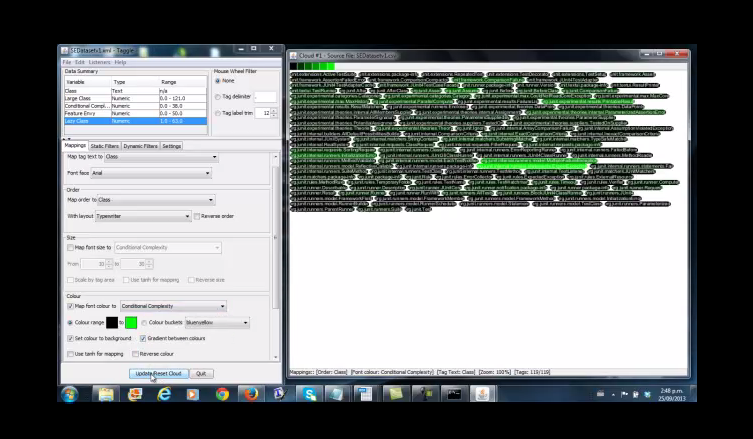
\includegraphics[scale=0.50]{distribution.png}
  \caption{\textit{Participant finding the data distribution for conditional complexity field, question T7}}
\end{subfigure}
\begin{subfigure}{\textwidth}
	\centering
 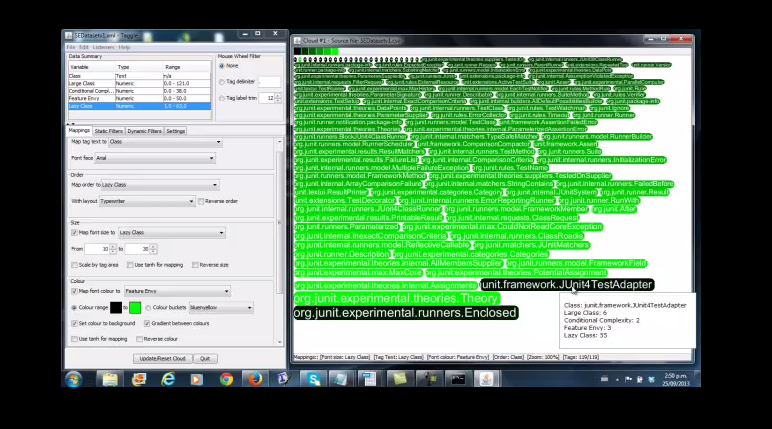
\includegraphics[scale=0.50]{outliers.png}
  \caption{\textit{Participant finding outliers in correlation between lazy class and feature envy, questions T6 and T8}}
\end{subfigure}
  \caption{\textit{Participants mapping font size and tag background colour to complete tasks}}
\label{fig:mapping}
\end{figure}


\paragraph{Legends, helpers and summary information}

We were interested in finding out more about particular areas of the interface which provided information to help the user in interpreting the visual encoding --- how much attention was paid to them, and how they were used. Those areas are as follows: \emph{legend} (the colour chip legend in the top left hand corner of the visual encoding, showing a sample colour for a variable numeric value), \emph{status bar} (the status bar at the bottom of the canvas showing what fields are mapped to which visual properties), \emph{details on demand} (pop-up screen supplying information about an individual record in the dataset), and the \emph{data summary screen} (the summary table describing ranges and data types for data fields in the dataset). Each area of interest is circled in Figure~\vref{fig:visualencoding}.

\begin{figure}[!htb]
\begin{subfigure}{.4\textwidth}
	\centering
  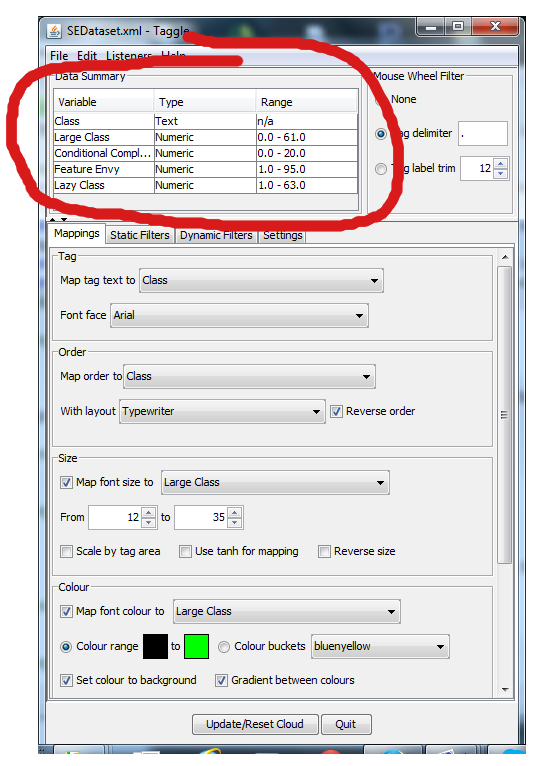
\includegraphics[scale=0.27]{interfacecircled.png}
\end{subfigure}%
\begin{subfigure}{.6\textwidth}
	\centering
 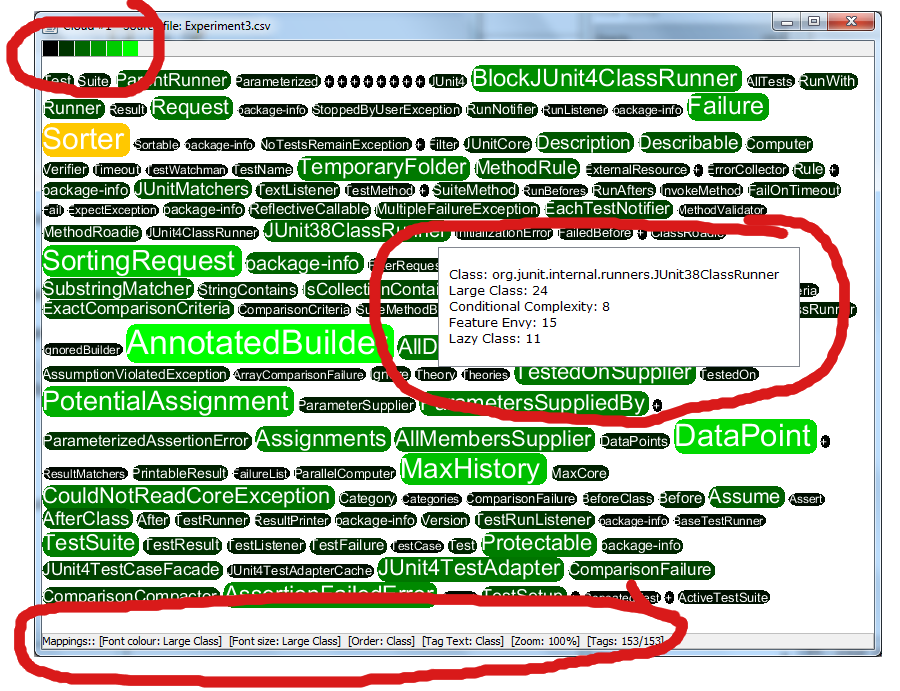
\includegraphics[scale=0.27]{visualencodingcircled.png}
\end{subfigure}
  \caption{\textit{Areas of interest circled (from top left to bottom right): data summary screen, legend, details on demand pop-up, status bar}}
\label{fig:visualencoding}
\end{figure}

Figure~\vref{fig:noofvisits} shows the participant average number of fixations and number of visits to each area of interest. Number of fixations is the total number of fixations that occur within an area of interest. Number of visits is the number of times participants looked at the area of interest -- there may be multiple fixations in the area of interest during a visit. (Note that automatically calculated metrics for details on demand pop-up screens could not be retrieved as they are user-initiated and do not appear constantly, or consistently in the same place on the interface). For the participants whose eye-tracking data was collected, no fixations or visits were made to the status bar. The colour chip legend had an average of one visit and fixation. This is generally because participants only used the default colour set when mapping to font colour, and only looked at the legend one time after first mapping to this visual property. We expect the colour chip legend would have received much more attention, had a categorical data field been included in the target dataset, as the user would have been required to look at the legend to find out which colour was mapped to which category. The data summary screen received the most attention with an average of 20 fixations within 13 visits. It appears users initially spent a lot of time assessing the data fields available within the dataset. 

\begin{figure}[!htb]
	\centering
	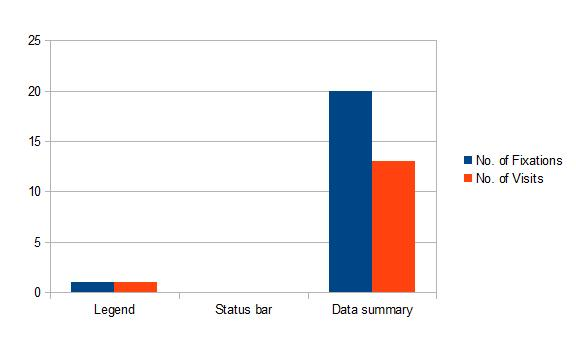
\includegraphics[scale=0.70]{noofvisits.jpg}
	\caption{\textit{Average number of fixations and number of visits to area of interest}}
	\label{fig:noofvisits}
\end{figure}

Figure~\vref{fig:totalvisitduration} shows the participant average of total duration of visits in seconds to the area of interest. In agreement with the number of fixations and durations spent in each area, the legend received an average of 0.28 seconds for all visits, the data summary screen received 4.87 seconds and the status bar received no visits. 

\begin{figure}[!htb]
	\centering
	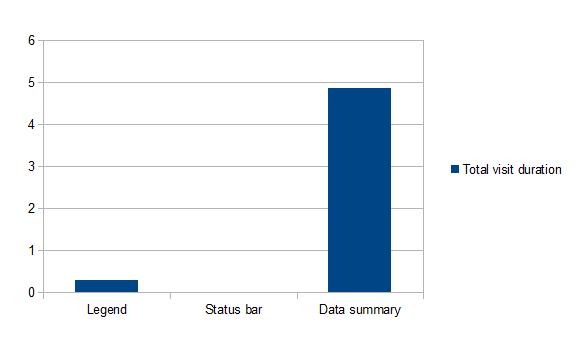
\includegraphics[scale=0.70]{totalvisitduration.jpg}
	\caption{\textit{Average total duration of visits to area of interest (in seconds)}}
	\label{fig:totalvisitduration}
\end{figure}

Details on demand pop-ups are different from the other three information sources in that some user action is required to use them whereas the others are nearly always visible (unless the data summary screen is contracted). Therefore, eye-gaze data for usage of pop-up details on demand had to be assessed manually. These pop-ups appear to be used much more frequently than any of the other three information sources.  Typical pop-up frequency (calculated from an indicative sample) is around four per minute, or about 75 for the whole of completion of experiment three. We suspect that the use of some of these are ``accidental'' --- this is because the default mouse mappings cause the pop-up to appear whenever the mouse rests over a tag.  (Initially we tried an explicit right-click action to display this pop-up, but during the heuristic evaluation detailed in Chapter~\ref{chap:heuristiceval} participants found it difficult to remember how to access this information).  For future work, we might consider logging the pop-up duration in order to distinguish deliberate and accidental pop-up display. Details on demand pop-ups were used particularly during classifying tasks such as T9 where users were asked to compare overall smelliness of particular classes (see Figure~\vref{fig:demandpopup} for examples) --- pop-up usage helped users discover information about other smells associated with the classes they were interested in.

\begin{figure}
	\centering
\begin{subfigure}{\textwidth}
	\centering
  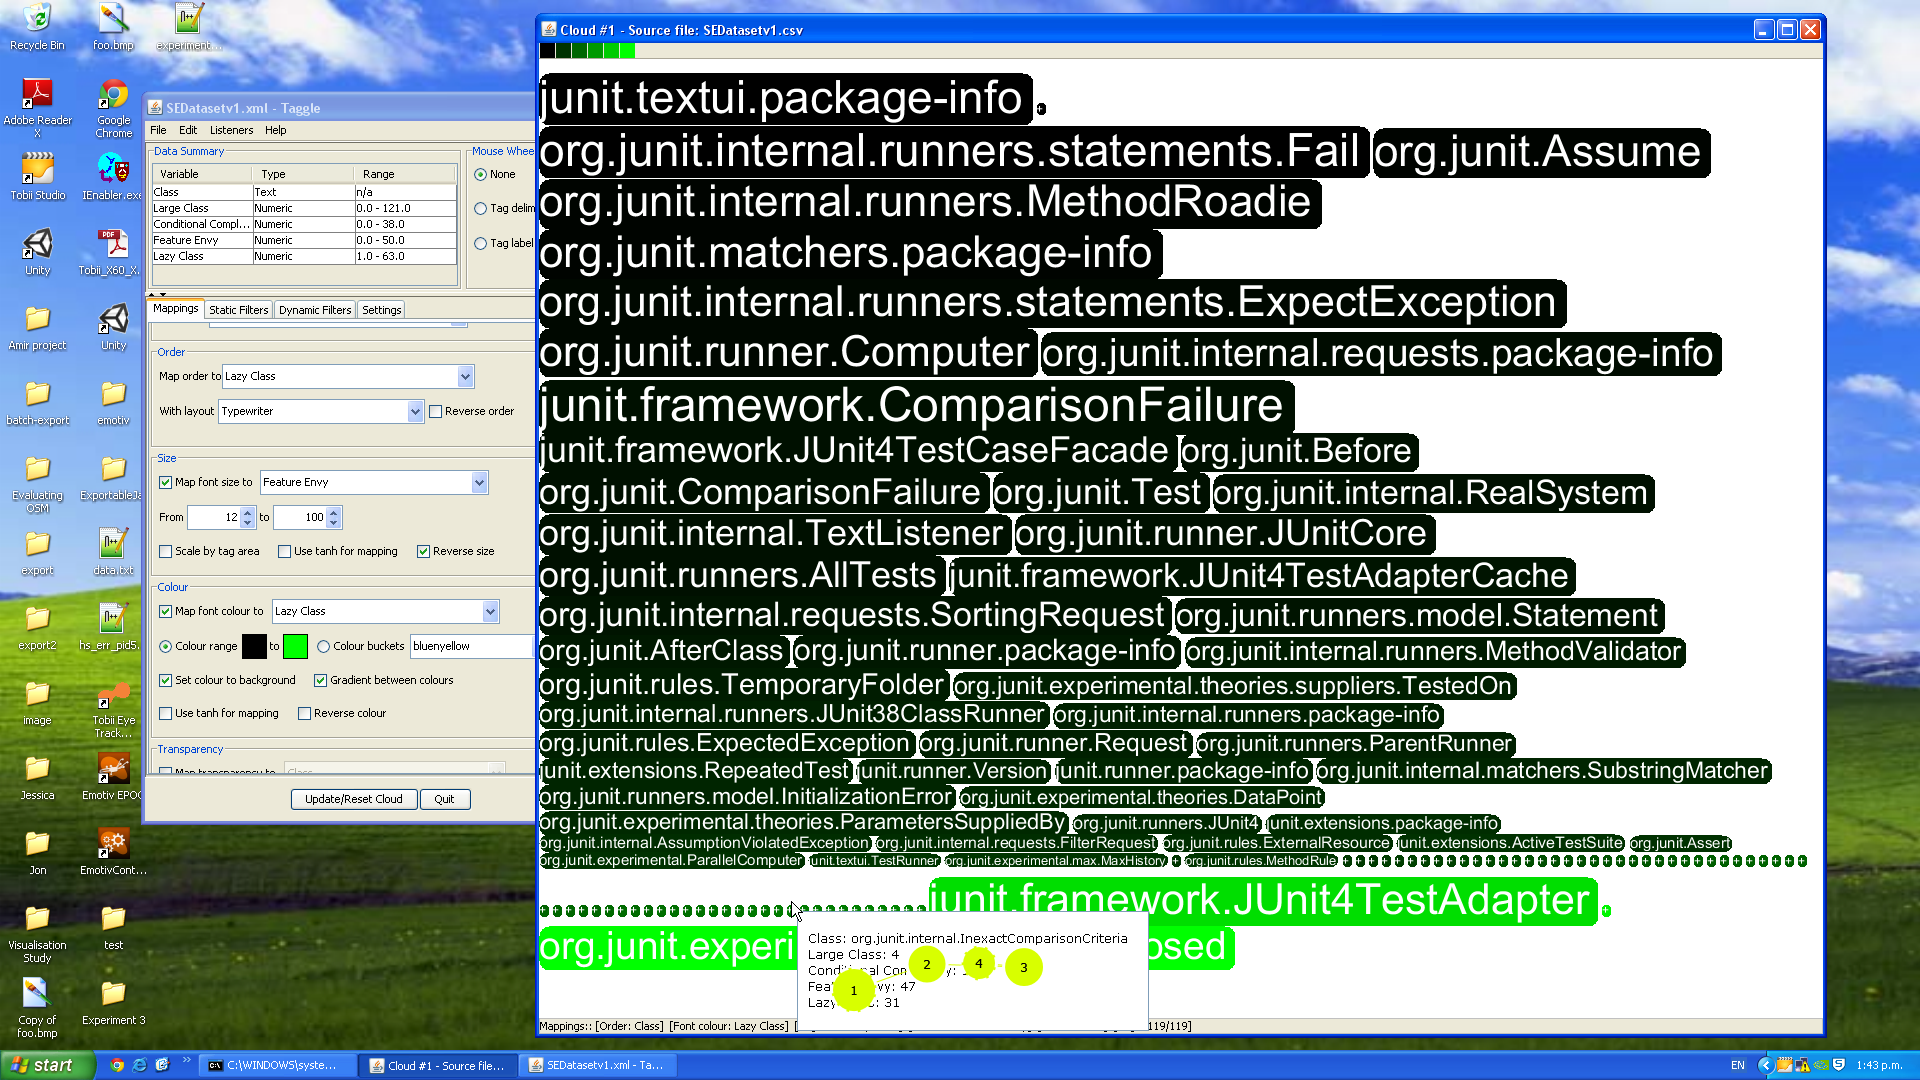
\includegraphics[scale=0.27]{popup1.png}
\end{subfigure}
\begin{subfigure}{\textwidth}
	\centering
 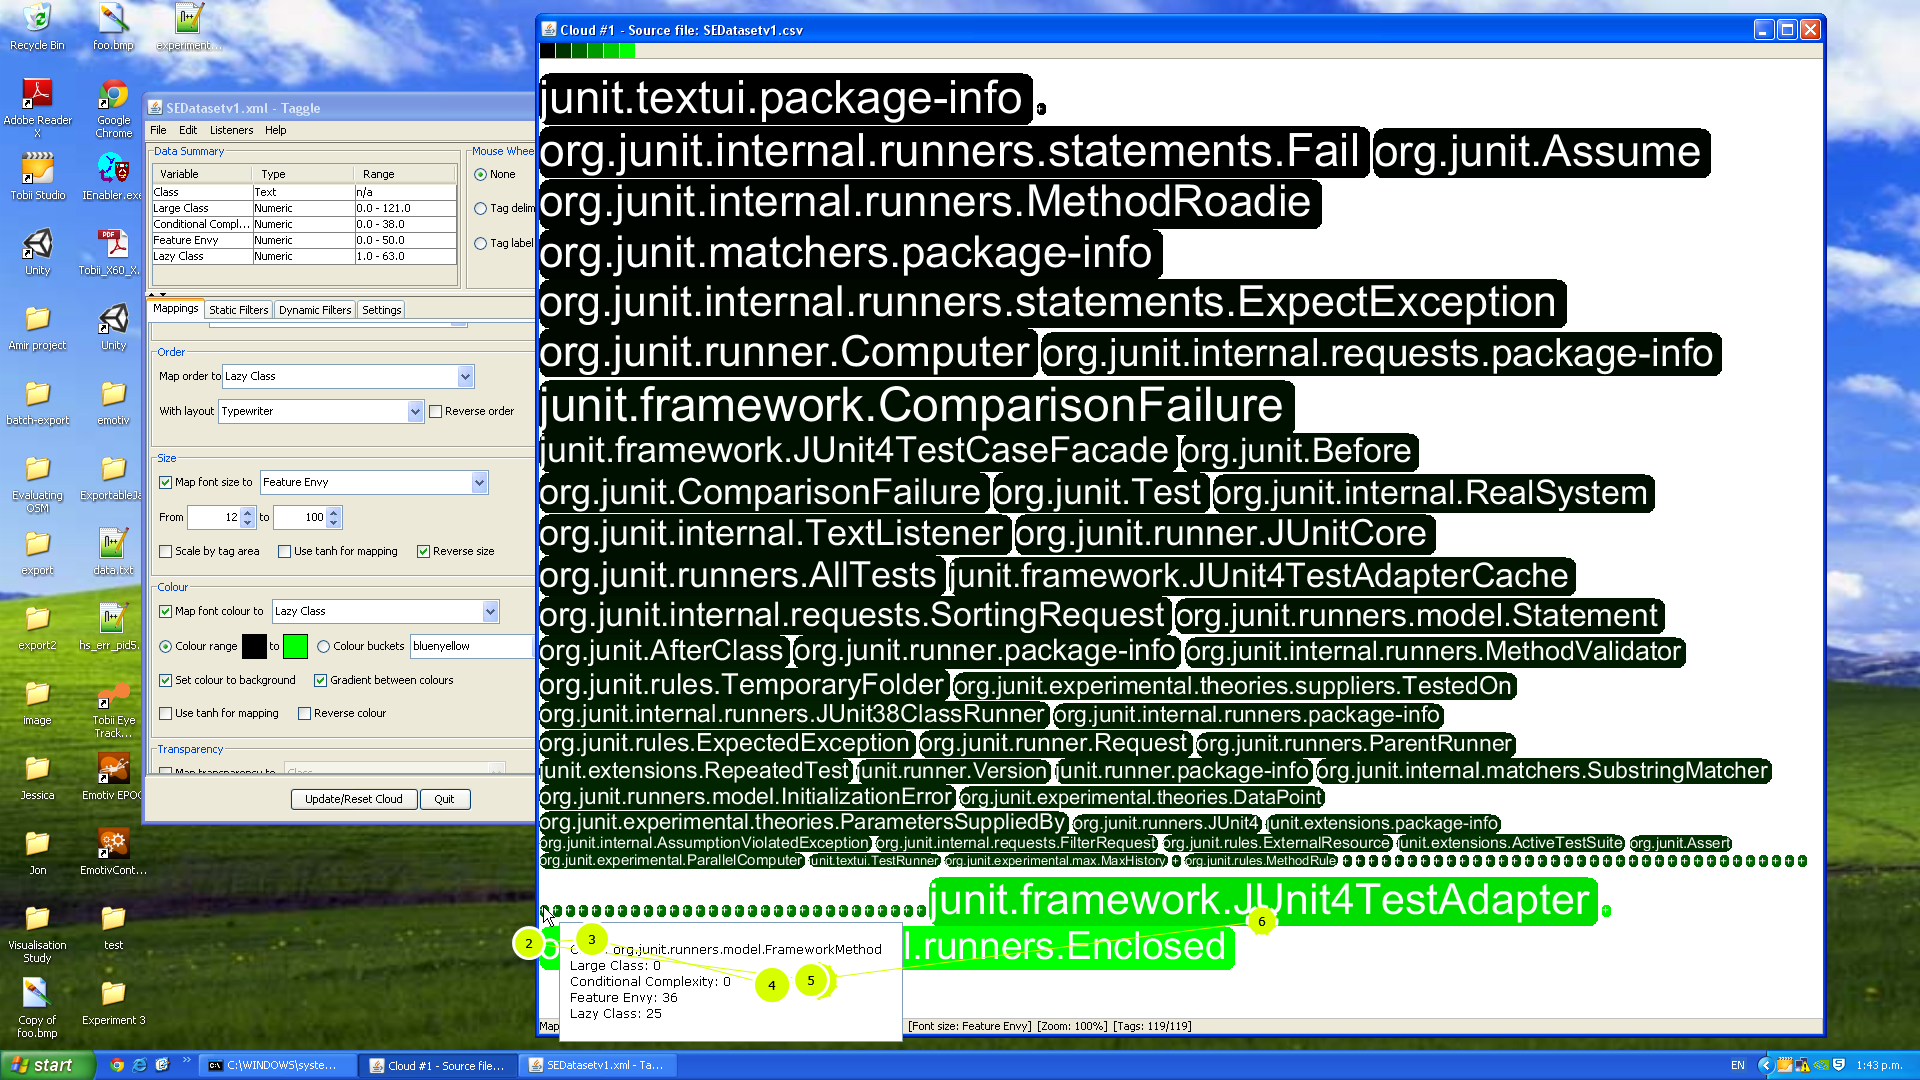
\includegraphics[scale=0.27]{popup2.png}
\end{subfigure}
  \caption{\textit{Eye-gaze on details on demand pop-up during question T9}}
\label{fig:demandpopup}
\end{figure}

\paragraph{Filtering}

The mouse wheel filtering was used by most participants. This was used to apply a tag delimiter filter to strip out package names of the classes and make the tag cloud size more managable. In Figure~\vref{fig:mousewheel}, the participant is in the process of applying the mouse wheel filter.

\begin{figure}[!htb]
	\centering
	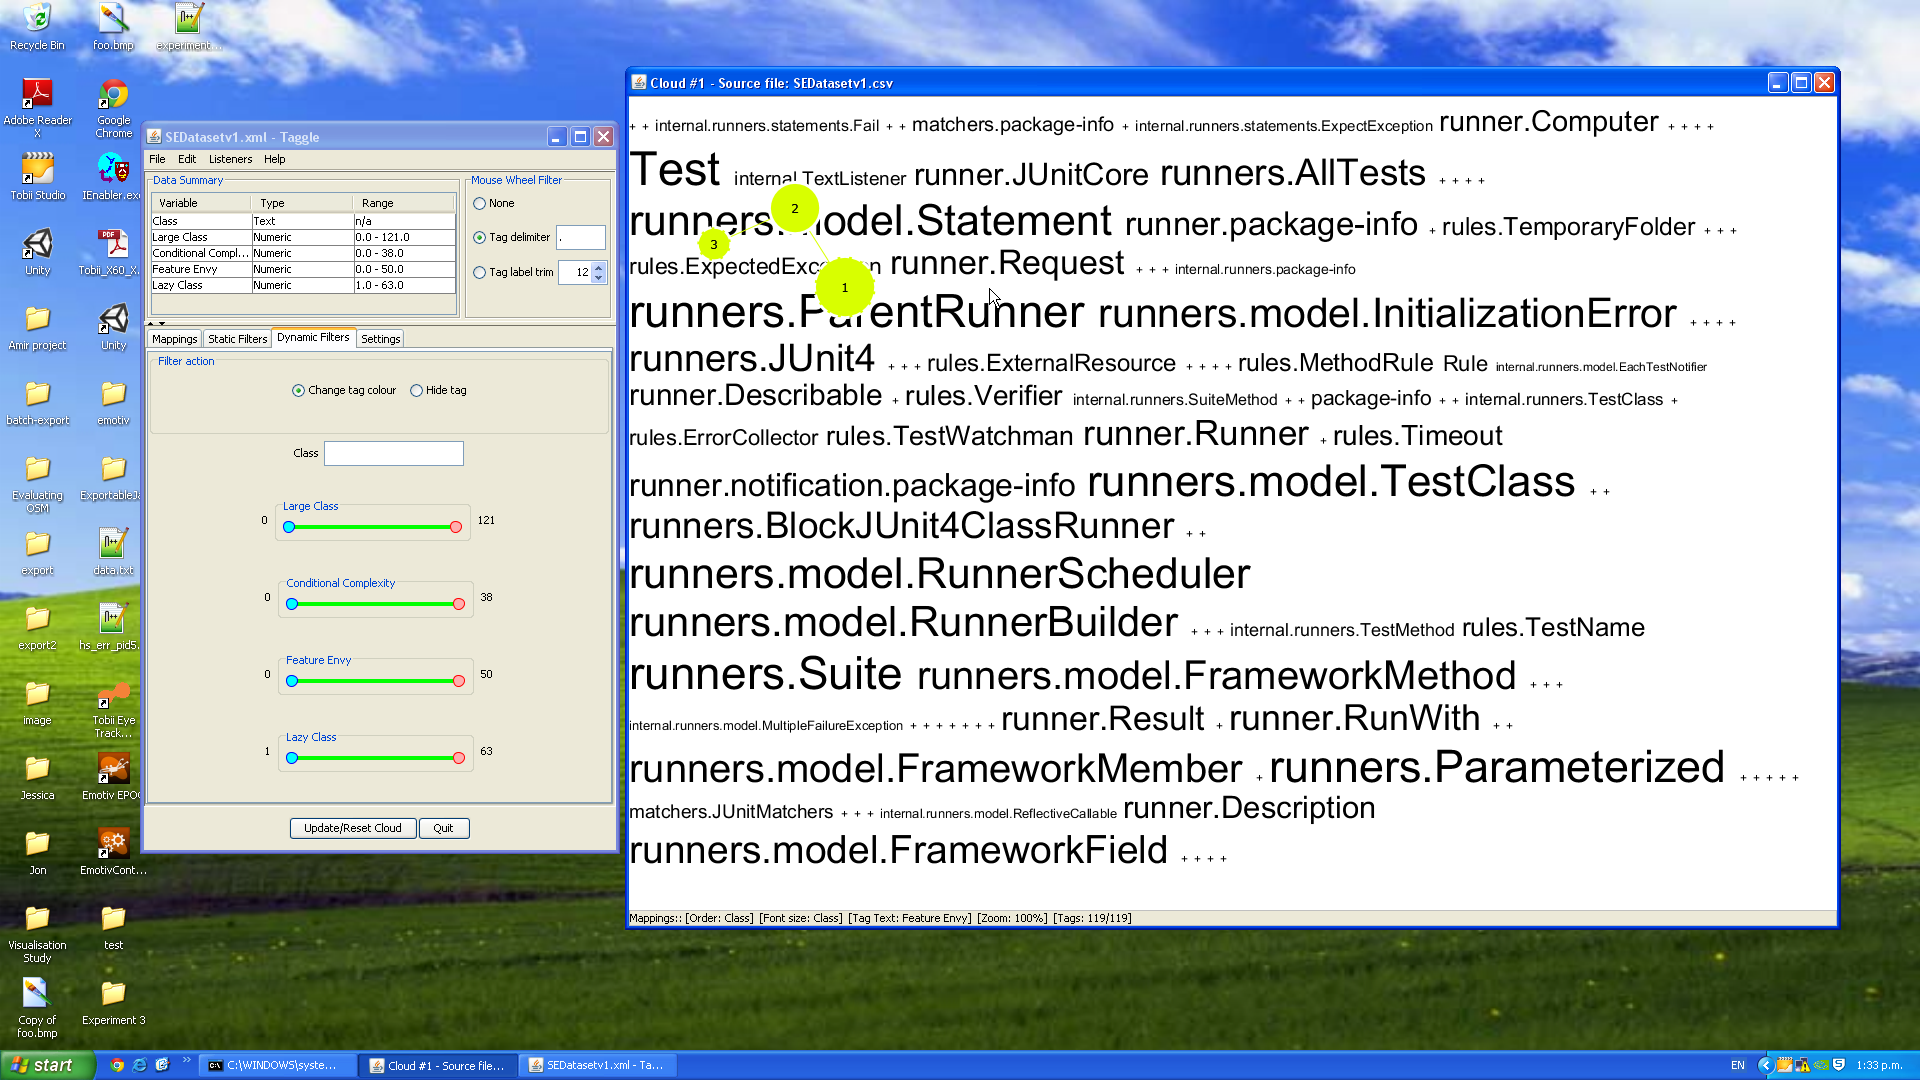
\includegraphics[scale=0.25]{mousewheelfilter.png}
	\caption{\textit{Participant is in the process of applying the mouse wheel filter to strip out package names}}
	\label{fig:mousewheel}
\end{figure}

Participants applied static filtering for questions which required specific information about tags, such as in clustering question T4 where users had to find information about classes from a particular package. Figure~\vref{fig:staticfiltering} shows a participant applying a static filter for question T4.

\begin{figure}[!htb]
	\centering
	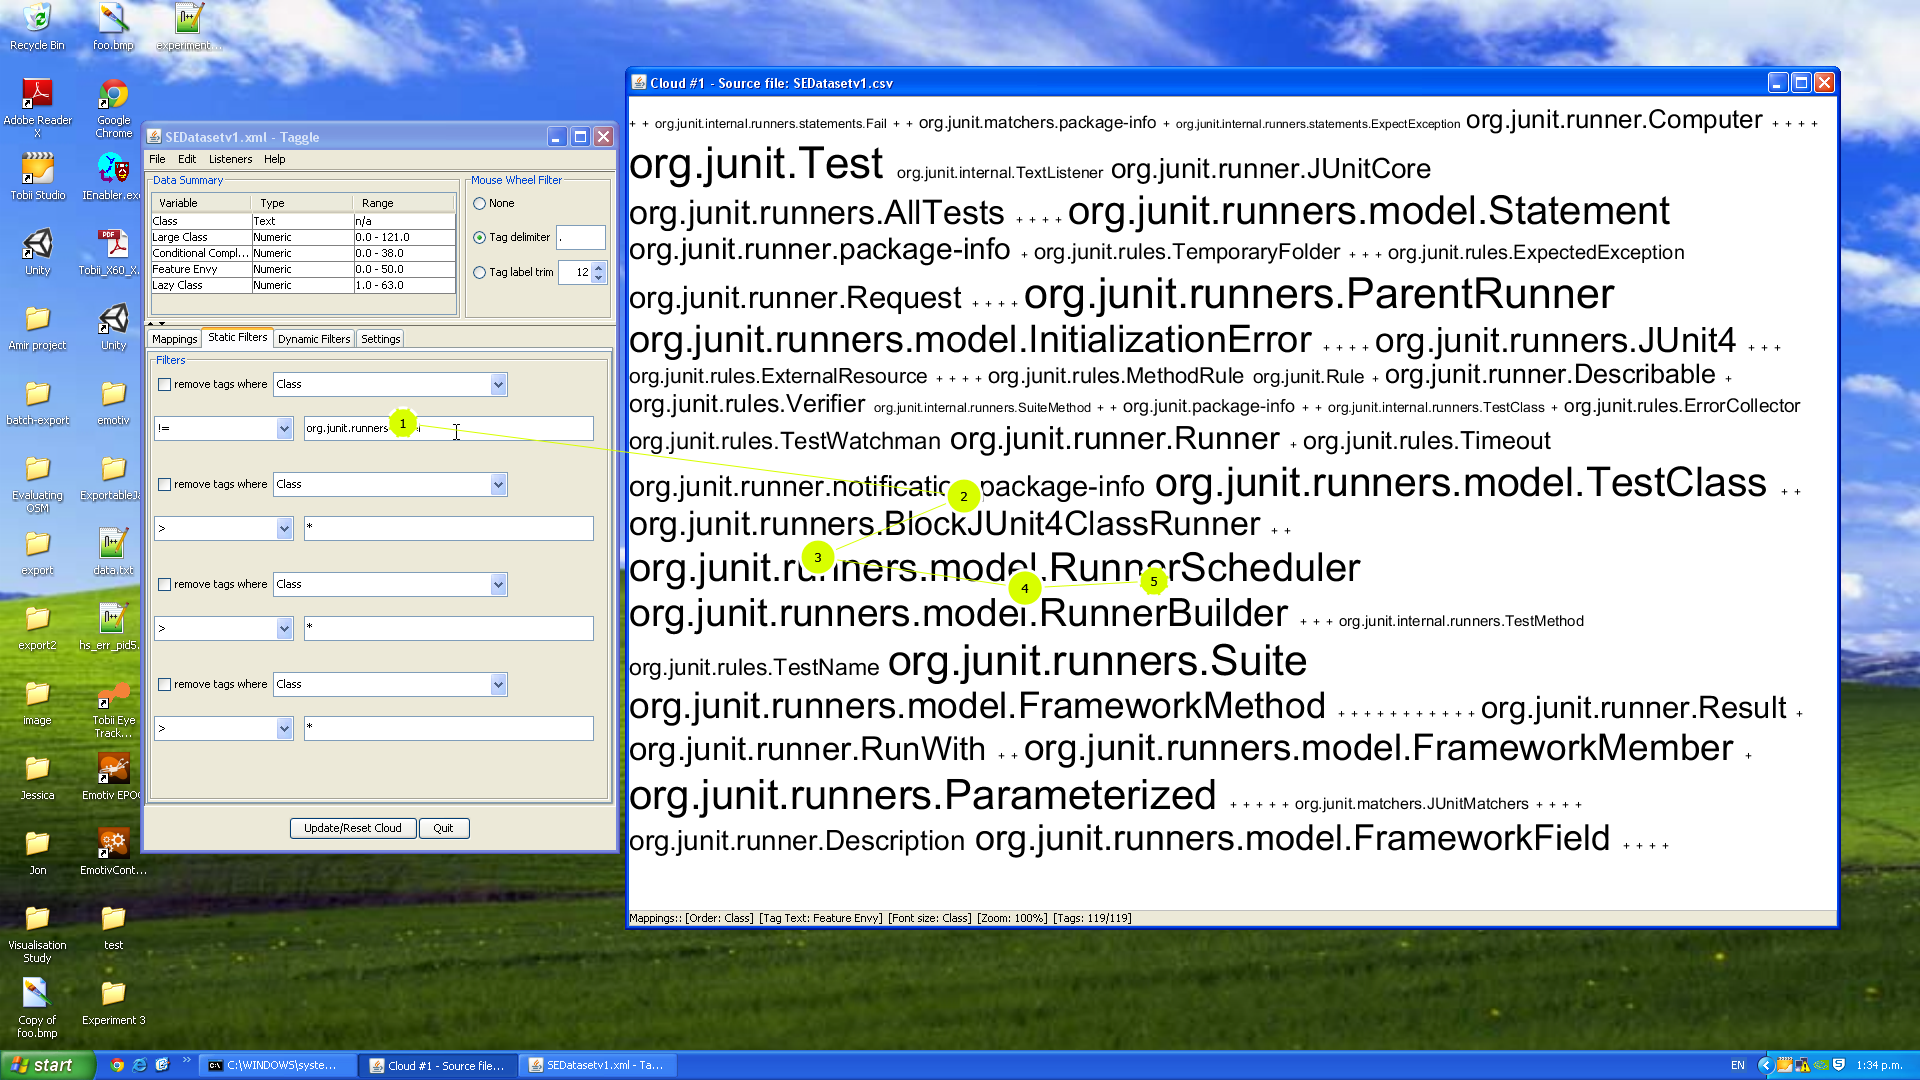
\includegraphics[scale=0.25]{staticfiltering.png}
	\caption{\textit{Participant has applied a static filter to locate particular classes in a package for question T4}}
	\label{fig:staticfiltering}
\end{figure}

Dynamic filtering was also applied by several participants when trying to find correlations between variables (T6), and when discovering information about classes with low values of a particular smell (T5 --- see Figure~\vref{fig:dynamicfilter}). 

\begin{figure}[!htb]
	\centering
	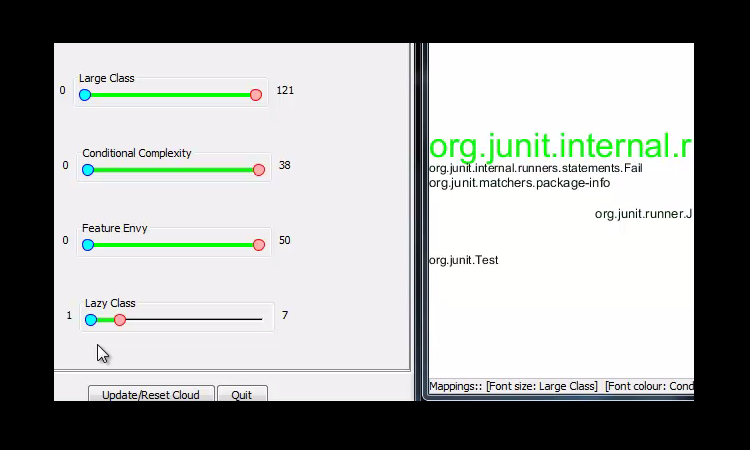
\includegraphics[scale=0.50]{dynamicfilter.png}
	\caption{\textit{Participant has applied a dynamic filter to locate classes low values of lazy class smell for question T5}}
	\label{fig:dynamicfilter}
\end{figure}


\subsection{Task analysis}

We defined three categories of answers for the tasks:
\begin{description}
\item[Correct answers:] the participant has given all correctly named classes, or explanations/illustrations of  relationships or patterns found.
\item[Partially correct answers:] the participant has given a subset of correctly named classes, or explanations/illustrations of relationships or patterns found.
\item[Incorrect/unanswered:] the participant has not answered the question, or has given an incorrect class name/explanation of relationships found. 
\end{description}

We interpreted the percentage of correct and partially correct answers of the participants as the extent to which the system is effective in facilitating data exploration and knowledge discovery in multidimensional software engineering data.

The numbers of correct, partially correct and incorrect answers for each task is presented in Table~\vref{tab:tasknumbers} and Figure~\vref{fig:resultstask} shows the percentage of correct and partially correct answers for each task. Only T5 and T7 had percentages of correct/partially correct answers below 80 percent. T1, identifying the class with the smelliest lazy class codesmell, was answered correctly by 83 percent of participants. Nearly 95 percent of participants were able to correctly identify at least one codesmell that a particular class had, and identify what class had no smell for feature envy. 

T4 was a more open-ended question, asking participants to state something about a particular package. In this case, the expected answer was to identify that classes from that package had very low values (0\textendash1) for code smells large class and conditional complexity. Participants were marked with a partially correct answer if they identified the package had low values for at least one of large class or conditional complexity. Over 80 percent of participants were able to identify at least one of the two low smell levels.

T5 was also an open-ended question which did not give the participants an exact description of the sort of answer that we expected. Participants were asked to state something about classes which contain low smelliness levels of lazy class. The expected response was to note they also contained low levels of feature envy. This led nicely to question T6 which queried as to what relationships they could find between variables. T5 had the lowest overall correct completion rate of all the tasks with only 66 percent answering correctly, while nearly 90 percent were able to identify at least one correlation between variables. Interestingly, some participants were able to identify the correlation between feature envy and lazy class without noticing that classes with low lazy class values had low feature envy values. It is possible question T5 was worded in a way that confused some participants.

T7 also had a lower rate of correct answers with only 66 percent of participants able to correctly identify a skewed data distribution of values for code smell large class. Ninety-five percent of participants were able to identify outliers in a correlation between two variables --- even participants who hadn't been able to identify any variable correlations in question T6. Finally, nearly 90 percent of participants were able to correctly compare two classes and identify which class was smelliest overall. 

\begin{table}
\centering
\caption{\textit{Number of correct, partially correct and incorrect answers}}
\begin{tabular}{|p{1cm}|p{3cm}|c|c|c|} \hline
 \textbf{Task} & \textbf{Task Type} &  \textbf{Correct} & \textbf{Partially correct} &\textbf{Incorrect}\\ \hline
T1	 & Classifying & 	15 & 	0 & 	3\\ \hline
T2	 & Classifying & 	16 & 	1 & 	1\\ \hline
T3	 & Classifying & 	17 & 	0 & 	1\\ \hline
T4	 & Clustering	 & 10 & 	5 & 	3\\ \hline
T5	 & Clustering & 	9 & 	3 & 	6\\ \hline
T6	 & Associative & 	16 & 	0 & 	2\\ \hline
T7	 & Summarising & 	12 & 	0 & 	6\\ \hline
T8	 & Summarising & 	17 & 	0 & 	1\\ \hline
T9	 & Classifying & 	16 & 	0 & 	2\\ \hline
\end{tabular}
\label{tab:tasknumbers}
\end{table}

\begin{figure}[!htb]
	\centering
	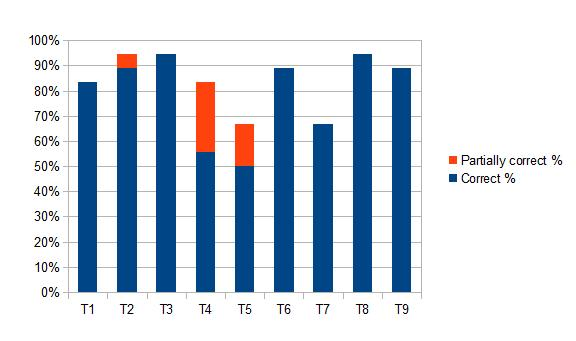
\includegraphics[scale=0.70]{resultstask.jpg}
	\caption{\textit{Percentage of correct and partially correct answers per task}}
	\label{fig:resultstask}
\end{figure}

Figure~\vref{fig:resultstasktype} shows the percentage of correct and partially correct answers for each task type category. The clustering tasks had the lowest overall percentage of correct answers as well the highest number of answers which were only partially correct.

\begin{figure}[!htb]
	\centering
	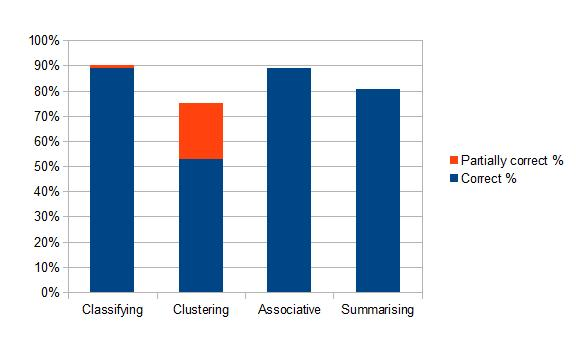
\includegraphics[scale=0.70]{resultstasktype.jpg}
	\caption{\textit{Percentage of correct and partially correct answers per task type}}
	\label{fig:resultstasktype}
\end{figure}

\section{Workload measures}

The NASA-TLX\citep{hart88} questionnaire is a multidimensional assessment used to rate perceived workload on six scales: mental demand, physical demand, temporal demand, performance, effort, and frustration. The scales are presented to participants as five 7-point scales with increments of high, medium and low estimates for each point (resulting in 21 gradations on the scales). This questionnaire was used to acquire subjective feedback on the perceived mental workload of the software engineering tasks. Figure~\vref{fig:nasatlx} shows the averaged results presented on a 7-point scale --- physical demand was perceived as very low (0.84), while mental demand and effort were the highest, rated 3.46 and 3.60 respectively. It can be noted that the averaged task indexes were perceived in the lower half of the scales for all workloads.

\begin{figure}[!htb]
	\centering
	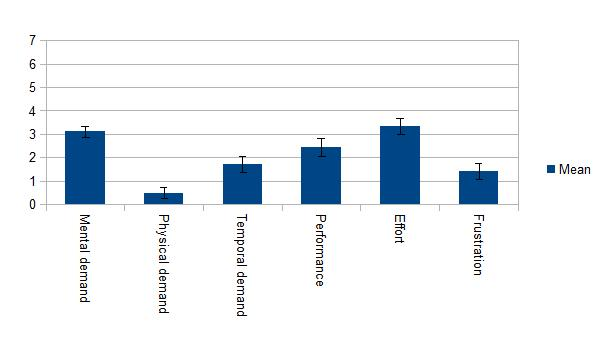
\includegraphics[scale=0.65]{nasatlx.jpg}
	\caption{\textit{NASA Task Load Index: perceived workload of Taggle on a 7-point scale (lower is better)}}
	\label{fig:nasatlx}
\end{figure}

\section{Summary and discussion}\label{sect:exp3summary}

Analysis of participant percentages of correct and partially correct answers for each task found that all tasks were completed between a 66 percent and 94 percent completion rate. Tasks which were performed the most poorly were tasks which asked the user to find classes which contained low levels of a particular code smell (T5) and discovery of the data distribution of another code smell (T7). Although this was briefly discussed during the software training, we query whether all participants had an understanding of the terms used in the questionnaire --- `skewed' and `normal' data distributions. The task which had the highest percentage of partially correct answers was T4, where participants where asked an open-ended question to state something about classes from a particular passage.

An analysis of tasks categorised into typical data mining categories (classification, clustering, association, summarising) found that clustering tasks performed the worst at a 74 percent successful completion rate, with the highest percentage of partially correct answers. We attribute this to the two clustering task questions being more open-ended than other questions (for example, `what can you tell me about classes from package ...'). This was because our goal was to see if participants could identify some similar characteristic of a group of tags. This open-ended nature of these questions resulted in some variation in answers. Both classifying and associative tasks had the highest percentage of successful answers at nearly 90 percent.

Eye-gaze and mouse-tracking data were analysed to find out how participants utilised the features in Taggle to complete tasks. Exploratory analysis showed participants who were able to successfully complete tasks used the rich interactive features in Taggle such as mapping multiple visual properties to data fields, and static and dynamic filtering. Participants who were not successfully able to complete a task tended to use inappropriate data mappings. Parts of the interface which showed summary data and information to help the user interpret the visual encoding were analysed to find out whether participants found them useful in the data exploration process. The data summary panel was identified as being highly used early in the exploration process to gain an overview of the underlying dataset. The data summary panel was included by request following results from our previous heuristic evaluation (see Chapter~\ref{chap:heuristiceval}). The mapping status bar was unused and the colour chip legend was used minimally. We expect that had the target dataset included categorical data, the colour chip legend would have been used more extensively so that users could find out which colours were mapped to particular categories. Pop-up details on demand for individual tags were also widely used for comparative or classifying tasks such as T9.

\begin{description}
\item[RQ:]\textit{Does Taggle support data exploration and knowledge discovery (discovery of relevant information) for software engineering data? How does it do this?} Overall, the task analysis and eye-tracking results were encouraging. Users had a generally high completion rate for all tasks (66 percent and over) and eye-gaze data showed users analysing and interpreting data using Taggle mappings for visual properties such as font size and colour. Interactive features such as filtering mechanisms to enable rich data exploration were also used.
\item[RQ:]\textit{Is the tool easy to learn? Can users manage to successfully complete typical software engineering tasks after a minimum or realistic amount of training?} We think the generally high task completion rates show that it is possible to take an interactive tag cloud visualisation tool such as Taggle, and have participants discover information about an unfamiliar dataset with a minimal ten minute training session. 
\end{description}

The study participants also completed a subjective assessment used to rate perceived workload (NASA-TLX). Averaged task indexes were perceived in the lower half of the 7-point scales for all workloads.

\section{Conclusion and future work}\label{sect:exp3conclusions}

Our results indicate the Taggle interactive tag cloud visualisation tool can be used by people with minimal training to discover relevant information about an unknown software engineering dataset. Experiment participants were able to effectively complete visual classification, clustering, association and summarising tasks to a generally high standard. Eye-gaze and mouse-tracking data showed participants utilising the interactive features of Taggle to analyse and interpret data.  The results of this study throw some interesting questions which could initiate future work --- further exploring the idea that a tag cloud interactive tool is easy to learn, including temporal data in our investigations, and looking into the usefulness of the data summary panel and details on demand pop-up in helping the user interpret the visual encoding. 

%Future work in this area could involve a comparative study comparing the effectiveness of knowledge discovery with Taggle against another tool.f



% ------------------------------------------------------------------------

%%% Local Variables: 
%%% mode: latex
%%% TeX-master: "../thesis"
%%% End: 
